\section{Operations}
\label{sec:related:ops}

Research on the analytical use of bus operational data spans three problem areas:
deriving quality-of-service indicators from vehicle telemetry, treating bus telemetry as
a city-wide traffic-sensing substrate, and short-horizon prediction of bus arrival times.
One peer-reviewed study informs the present project in each area; the
constructions each study contributes are taken up in the design chapters
that follow.

\subsection{QoS Indicators}
\label{sec:related:ops:qos}

Srisakaokul and colleagues \cite{srisakaokul2023} study the Bangkok city bus network and
propose three Quality of Service (QoS) indicators that are computed independently from
raw vehicle telemetry. The three indicators decompose service quality along three axes:
trip completion (whether a scheduled trip is executed end to end), path adherence
(whether the vehicle remains on the published route), and schedule adherence (whether
each scheduled passage at a stop occurs within an acceptable time band). The study is
offline; the indicators are reported as descriptive statistics across the studied fleet
rather than as inputs to a real-time alerting system.

Figure~\ref{fig:related:qos} illustrates the three indicators on a
stylised route trajectory.

\begin{figure}[!htbp]
\centering
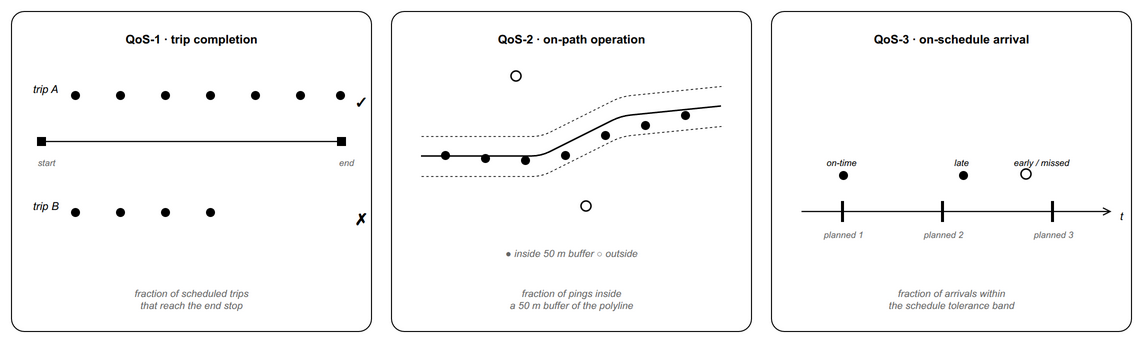
\includegraphics[width=0.96\linewidth]{images/diagrams/related_qos_panels.png}
\caption{The three QoS indicators on a stylised route trajectory.}
\label{fig:related:qos}
\end{figure}

The principal methodological contribution of the study, from the point
of view of the present project, is the decision to report the three
axes separately rather than as a single composite score. A composite
score collapses information; reporting the three axes side by side
preserves the information and allows a reader to see which axis of
service quality a given route is weak on. Section \ref{sec:foundations:qos} of the
present report develops the QoS framework in technical detail, with explicit definitions
of each indicator and the geometric tolerances used to compute them. Section
\ref{sec:solution:viz} adopts the framework as the data source for the reliability
indicators of one of the analytical themes of the proposed system.

\subsection{Telemetry Sensing}
\label{sec:related:ops:sensing}

Derevitskiy and colleagues \cite{derevitskiy2016} present an aggregate-based method that
treats the urban bus fleet as a distributed traffic-sensing substrate. The method
aggregates raw GPS pings emitted by the bus fleet into edge-speed estimates over the
city's road graph; where no bus currently operates on a given road segment, the method
propagates an estimate from neighbouring segments using a macroscopic travel-time model
that incorporates the effect of traffic signals and the time of day. The reported mean
absolute percentage error is approximately 20 percent at distances under 15 kilometres,
which the authors argue is acceptable for many planning-support applications.

The construction is relevant to the present project because the same GPS feed used to
compute the reliability indicators of Section \ref{sec:related:ops:qos} could, in
principle, be used to derive a city-wide traffic-speed map at no additional data cost.
The Phase One scope of the present project does not implement this construction; the
construction is recorded in Chapter \ref{chapter:future} as a candidate extension that
becomes feasible once the full GPS time window of the source dataset is available for
processing.

\subsection{Arrival Prediction}
\label{sec:related:ops:arrival}

Lin and Zeng \cite{linzeng2014} build a real-time predictor for bus arrival times at
downstream stops. The construction proceeds in three steps. First, each vehicle's raw
GPS pings are projected onto the one-dimensional path of the route the vehicle is
operating, yielding a per-trip time-distance trajectory. Second, the trajectory is
extrapolated forward in time using a model that combines free-flow speed with stop-level
dwell time. Third, the predicted arrival time at each downstream stop is read off the
extrapolated trajectory. The study reports that dwell time at time-check stops is the
dominant predictor of arrival error; free-flow speed varies relatively little between
trips on the same route.

Two ideas from the study transfer to the present project. The first is the construction
of a per-trip time-distance trajectory, which serves as the data primitive behind one of
the visualisation primitives catalogued in the present report (see Section
\ref{sec:foundations:primitives}). The second is the empirical observation that
stop-level dwell time carries an unusually large share of the variance in arrival error;
this observation motivates the inclusion of stop-level dwell measurement among the
operational quantities surfaced by the proposed system.
